\documentclass[12pt,a4paper]{report}

\usepackage[margin=1in]{geometry}
\usepackage[T1]{fontenc}
\usepackage[utf8]{inputenc}
\usepackage{lmodern}
\usepackage{setspace}
\usepackage{booktabs}
\usepackage{array}
\usepackage{longtable}
\usepackage{hyperref}
\usepackage{xcolor}
\usepackage{float}
\usepackage{listings}
\usepackage{tikz}
\usetikzlibrary{arrows.meta, positioning, shapes.geometric, shapes.multipart}

\hypersetup{
    colorlinks=true,
    linkcolor=blue!50!black,
    urlcolor=blue!50!black,
    citecolor=blue!50!black
}

\onehalfspacing
\setlength{\parskip}{0.5em}
\setlength{\parindent}{0pt}

\lstdefinestyle{reportcode}{
    basicstyle=\ttfamily\small,
    backgroundcolor=\color{gray!8},
    frame=single,
    breaklines=true,
    showstringspaces=false,
    columns=fullflexible
}

\title{Academic Report on a Library Borrowing Management System}
\author{
    Student Name: [Your Name] \\
    Student ID: [Your ID] \\
    Course: [Course Title] \\
    Department: [Department Name]
}
\date{April 26, 2026}

\begin{document}

\begin{titlepage}
    \centering
    \vspace*{2cm}
    {\Large [University Name]\par}
    \vspace{1.5cm}
    {\Huge\bfseries Academic Report on a Library Borrowing Management System\par}
    \vspace{1cm}
    {\Large Design, Transactional Behavior, and Integration Testing\par}
    \vfill
    \begin{tabular}{>{\bfseries}l l}
        Student Name: & [Your Name] \\
        Student ID: & [Your ID] \\
        Course Title: & [Course Title] \\
        Instructor: & [Instructor Name] \\
        Submission Date: & April 26, 2026 \\
    \end{tabular}
    \vfill
\end{titlepage}

\pagenumbering{roman}
\tableofcontents
\clearpage

\chapter*{Abstract}
\addcontentsline{toc}{chapter}{Abstract}
This report presents the design and testing analysis of a small Java-based Library Borrowing Management System implemented with Spring Boot, JDBC, and MySQL. The system supports two core business operations: borrowing a book and returning a book. Its architecture separates business logic from data access through a layered design consisting of service, DAO, and persistence layers. The report explains the implementation structure, conceptual data model, and transactional behavior of the system. It also documents the integration test suite executed through Maven, including observed outputs and test results. The experimental execution confirmed that all three provided test cases passed successfully, validating stock updates, borrowing record insertion, and return record modification. A limitation is also identified: the current rollback-oriented test verifies failure behavior before a partial update occurs, rather than forcing an exception after a database write. This means the application structure is appropriate for demonstrating transaction-oriented service logic, but the rollback evidence could be strengthened further in future work.

\textbf{Keywords:} Spring Boot, JDBC, MySQL, Maven, Integration Testing, Transactions, Library Management System

\clearpage
\pagenumbering{arabic}

\chapter{Introduction}
Software systems used in academic and administrative settings often require reliable transaction handling because data consistency is essential. A library management scenario is a common example: when a book is borrowed, the available stock must decrease and a borrowing record must be inserted as part of one logical operation. Similarly, when a book is returned, the stock must increase and the latest borrowing record must be updated to indicate return completion.

The project analyzed in this report implements these operations in Java using Spring Boot and JDBC. The codebase is intentionally compact, which makes it suitable for academic explanation. Even so, it demonstrates several important enterprise software concepts, including layered design, dependency injection, transaction demarcation, relational persistence, and automated testing.

The purpose of this report is fourfold:
\begin{enumerate}
    \item to explain the architectural structure of the project;
    \item to describe the core borrowing and returning workflows;
    \item to document the observed integration test execution and output; and
    \item to evaluate strengths and limitations of the current implementation.
\end{enumerate}

\chapter{Project Overview}

\section{Technology Stack}
The project is configured as a Maven application. The main dependencies declared in the build configuration establish a Spring Boot application with JDBC-based persistence and a MySQL runtime driver.

\begin{table}[H]
    \centering
    \caption{Primary technologies used in the project}
    \begin{tabular}{p{4cm} p{8.5cm}}
        \toprule
        \textbf{Component} & \textbf{Role in the Project} \\
        \midrule
        Java 17 & Programming language and runtime platform \\
        Spring Boot 3.3.0 & Application bootstrap, dependency injection, testing support \\
        Spring JDBC & Simplified database access through \texttt{JdbcTemplate} \\
        MySQL Connector/J & Runtime connectivity to the MySQL database \\
        Maven & Build, dependency management, and test execution \\
        JUnit 5 / Spring Boot Test & Integration testing framework \\
        \bottomrule
    \end{tabular}
\end{table}

\section{Functional Scope}
The implemented system supports two main use cases:
\begin{enumerate}
    \item \textbf{Borrow a book}: verify the book exists, confirm stock is available, decrease stock, and insert a borrowing record.
    \item \textbf{Return a book}: identify the most recent active borrowing record, increase stock, and mark the record as \texttt{RETURNED}.
\end{enumerate}

The business logic is exposed through the \texttt{LibraryService} interface and concretely implemented in \texttt{LibraryServiceImpl}. Both methods are annotated with \texttt{@Transactional}, which makes the service layer responsible for preserving consistency across multiple database operations.

\chapter{System Design and Architecture}

\section{Layered Architecture}
The project follows a clear layered architecture. The test suite invokes the service layer; the service layer coordinates domain operations; the DAO layer executes SQL statements; and MySQL stores the persistent data.

\begin{figure}[H]
    \centering
    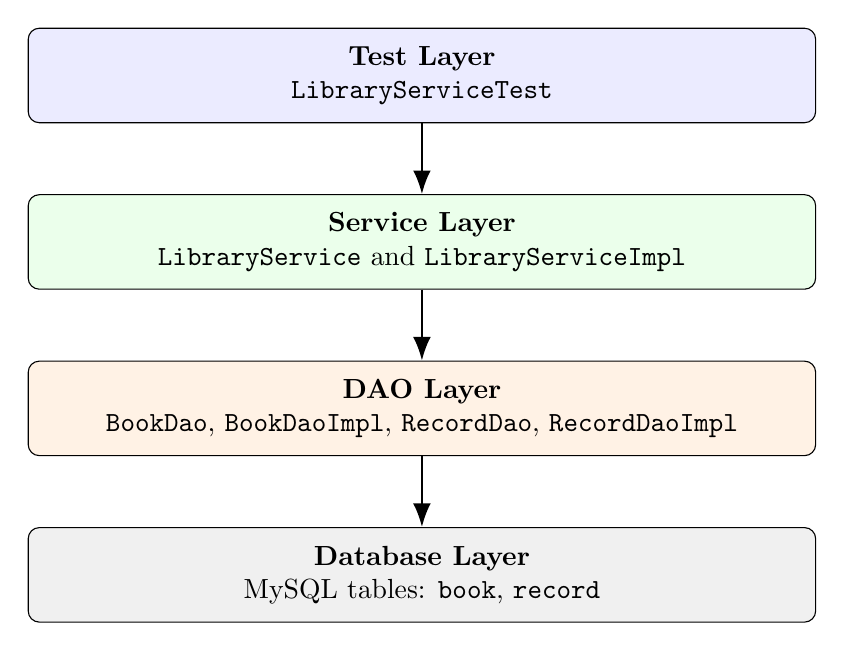
\begin{tikzpicture}[
        box/.style={
            draw,
            rounded corners,
            minimum width=10cm,
            minimum height=1.2cm,
            align=center,
            fill=blue!8
        },
        arrow/.style={-{Latex[length=3mm]}, thick}
    ]
        \node[box] (test) {\textbf{Test Layer} \\ \texttt{LibraryServiceTest}};
        \node[box, below=0.9cm of test, fill=green!8] (service) {\textbf{Service Layer} \\ \texttt{LibraryService} and \texttt{LibraryServiceImpl}};
        \node[box, below=0.9cm of service, fill=orange!10] (dao) {\textbf{DAO Layer} \\ \texttt{BookDao}, \texttt{BookDaoImpl}, \texttt{RecordDao}, \texttt{RecordDaoImpl}};
        \node[box, below=0.9cm of dao, fill=gray!12] (db) {\textbf{Database Layer} \\ MySQL tables: \texttt{book}, \texttt{record}};

        \draw[arrow] (test) -- (service);
        \draw[arrow] (service) -- (dao);
        \draw[arrow] (dao) -- (db);
    \end{tikzpicture}
    \caption{Layered architecture of the Library Borrowing Management System}
\end{figure}

\section{Main Classes and Responsibilities}
\begin{longtable}{p{4.2cm} p{9.5cm}}
    \caption{Principal classes and their responsibilities} \\
    \toprule
    \textbf{Class / Interface} & \textbf{Responsibility} \\
    \midrule
    \endfirsthead
    \toprule
    \textbf{Class / Interface} & \textbf{Responsibility} \\
    \midrule
    \endhead
    \texttt{LibraryApplication} & Entry point that starts the Spring Boot application context. \\
    \texttt{LibraryService} & Service interface defining \texttt{borrowBook} and \texttt{returnBook}. \\
    \texttt{LibraryServiceImpl} & Transactional business implementation that coordinates DAO operations. \\
    \texttt{BookDao} / \texttt{BookDaoImpl} & Inserts books, updates stock, and retrieves books by name. \\
    \texttt{RecordDao} / \texttt{RecordDaoImpl} & Inserts records, lists records, finds the most recent borrowed record, and updates record status. \\
    \texttt{Book} & Domain object containing \texttt{id}, \texttt{name}, and \texttt{stock}. \\
    \texttt{Record} & Domain object containing \texttt{id}, \texttt{bookName}, \texttt{borrower}, and \texttt{status}. \\
    \texttt{LibraryServiceTest} & Spring Boot integration test class validating the major business scenarios. \\
    \bottomrule
\end{longtable}

\section{Conceptual Data Model}
The source code implies a relational model centered on two tables: \texttt{book} and \texttt{record}. Although schema creation scripts are not included in the project, the SQL statements used by the DAOs allow the structure to be inferred reliably.

\begin{figure}[H]
    \centering
    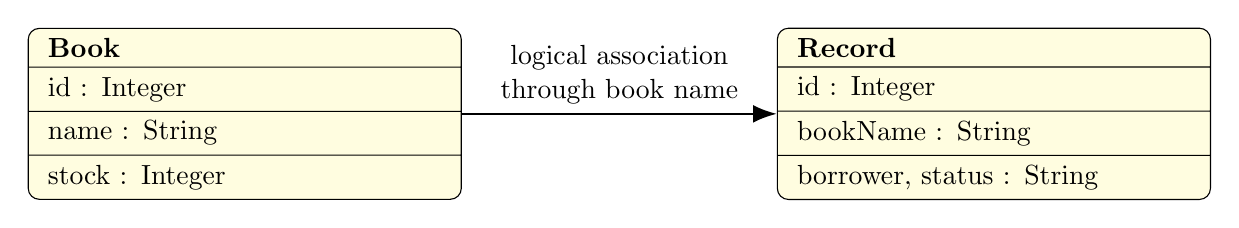
\begin{tikzpicture}[
        entity/.style={
            draw,
            rectangle split,
            rectangle split parts=4,
            rounded corners,
            minimum width=5.5cm,
            fill=yellow!12,
            text width=5cm
        },
        relarrow/.style={-{Latex[length=3mm]}, thick}
    ]
        \node[entity] (book) {
            \textbf{Book}
            \nodepart{second} id : Integer
            \nodepart{third} name : String
            \nodepart{fourth} stock : Integer
        };

        \node[entity, right=4cm of book] (record) {
            \textbf{Record}
            \nodepart{second} id : Integer
            \nodepart{third} bookName : String
            \nodepart{fourth} borrower, status : String
        };

        \draw[relarrow] (book) -- node[above, align=center] {logical association\\through book name} (record);
    \end{tikzpicture}
    \caption{Conceptual entity relationship inferred from DAO operations}
\end{figure}

It is important to note that the current implementation links records to books through the textual field \texttt{book\_name} rather than through a foreign key to \texttt{book.id}. This is acceptable for a small demonstration system, but in a production-grade design a direct foreign-key relationship would normally be preferable.

\chapter{Transactional Workflow}

\section{Borrowing Process}
The borrowing process is implemented in the service layer as a transaction. Its logical sequence can be summarized as follows:
\begin{enumerate}
    \item retrieve the requested book by name;
    \item reject the request if the book does not exist;
    \item reject the request if the stock is zero or negative;
    \item decrease the stock by one; and
    \item insert a new record with status \texttt{BORROWED}.
\end{enumerate}

\begin{figure}[H]
    \centering
    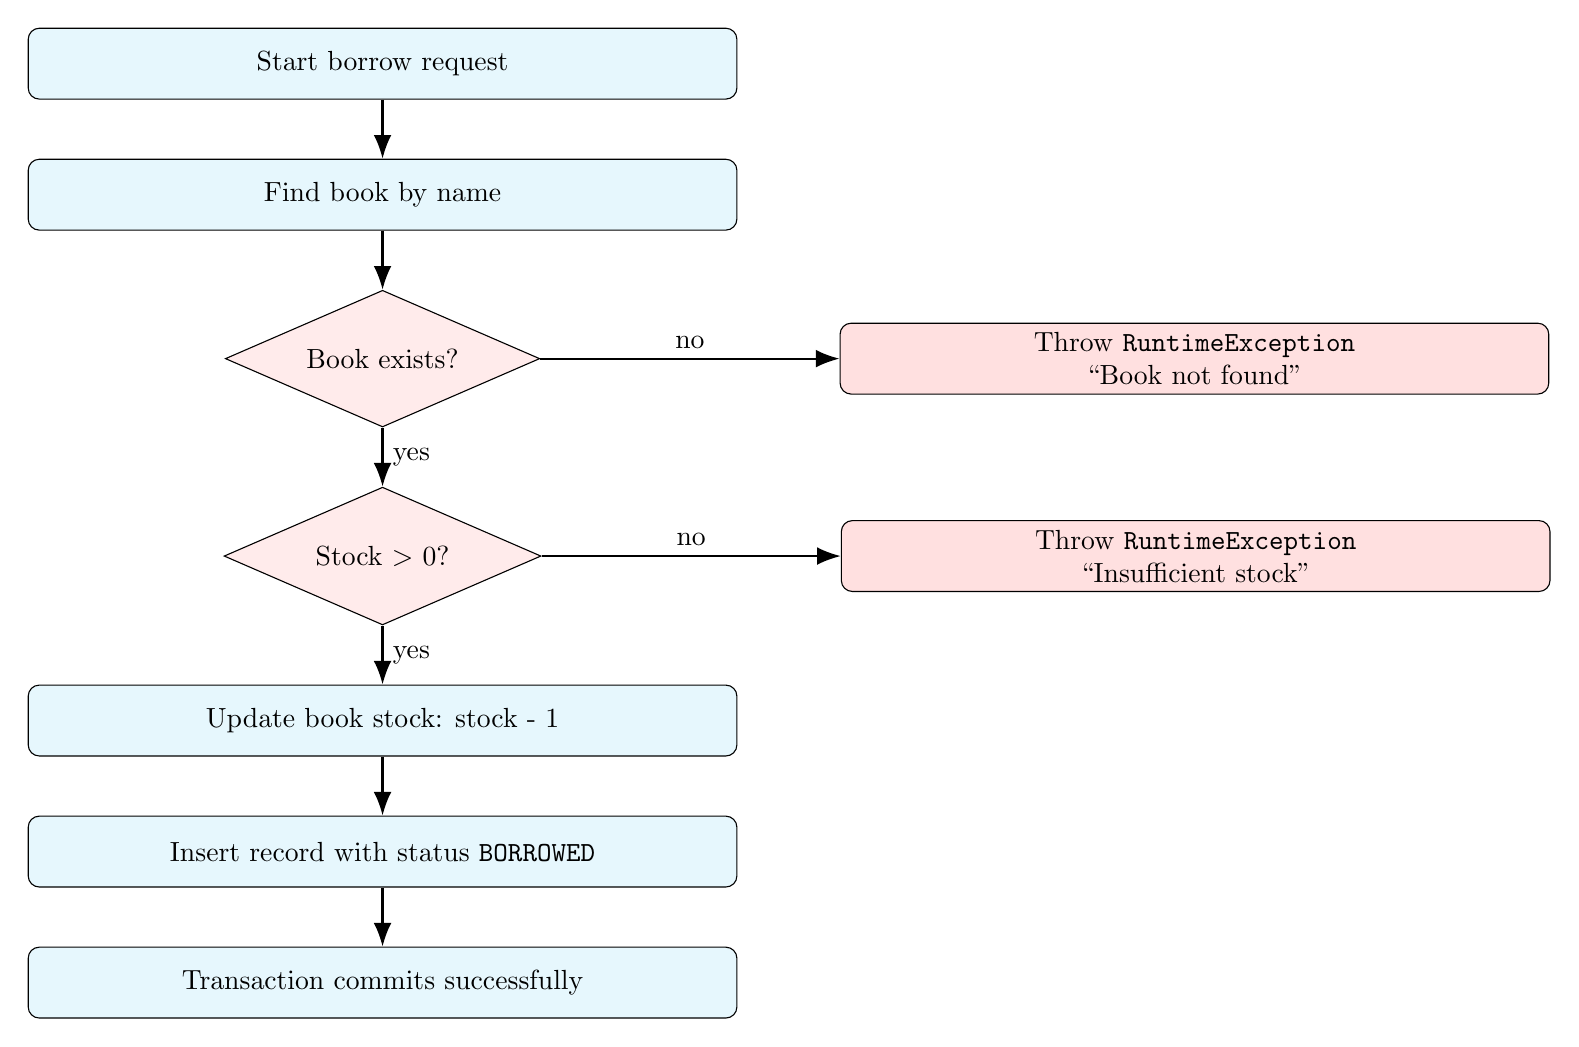
\begin{tikzpicture}[
        node distance=0.75cm,
        flow/.style={
            draw,
            rounded corners,
            align=center,
            minimum width=9cm,
            minimum height=0.9cm,
            fill=cyan!10
        },
        decision/.style={
            draw,
            diamond,
            aspect=2.3,
            align=center,
            fill=red!8,
            text width=3.2cm,
            inner sep=1pt
        },
        arrow/.style={-{Latex[length=3mm]}, thick}
    ]
        \node[flow] (start) {Start borrow request};
        \node[flow, below=of start] (find) {Find book by name};
        \node[decision, below=of find] (exists) {Book exists?};
        \node[decision, below=of exists] (stock) {Stock $>$ 0?};
        \node[flow, below=of stock] (update) {Update book stock: stock - 1};
        \node[flow, below=of update] (record) {Insert record with status \texttt{BORROWED}};
        \node[flow, below=of record] (commit) {Transaction commits successfully};

        \node[flow, right=3.8cm of exists, fill=red!12] (missing) {Throw \texttt{RuntimeException}\\``Book not found''};
        \node[flow, right=3.8cm of stock, fill=red!12] (nostock) {Throw \texttt{RuntimeException}\\``Insufficient stock''};

        \draw[arrow] (start) -- (find);
        \draw[arrow] (find) -- (exists);
        \draw[arrow] (exists) -- node[right] {yes} (stock);
        \draw[arrow] (stock) -- node[right] {yes} (update);
        \draw[arrow] (update) -- (record);
        \draw[arrow] (record) -- (commit);
        \draw[arrow] (exists.east) -- node[above] {no} (missing.west);
        \draw[arrow] (stock.east) -- node[above] {no} (nostock.west);
    \end{tikzpicture}
    \caption{Borrowing workflow implemented by the service layer}
\end{figure}

\section{Returning Process}
The return operation is also transactional. It looks up the book, retrieves the latest active borrowing record for the specified borrower, increments the stock, and updates that record's status to \texttt{RETURNED}. This approach keeps the logic simple and consistent with the educational scope of the project.

\chapter{Testing Methodology}

\section{Nature of the Test Suite}
The class \texttt{LibraryServiceTest} is an integration test annotated with \texttt{@SpringBootTest}. This means the tests load the Spring application context and interact with the actual configured database through the DAOs and \texttt{JdbcTemplate}. The testing strategy therefore validates end-to-end service behavior rather than isolated unit-level method calls.

\section{Database Preconditions}
The test configuration points to a MySQL database using a local JDBC URL. The database initialization mode is disabled, which means the database schema must already exist before the test suite is executed. The test setup deletes all rows from the \texttt{record} and \texttt{book} tables before each test and then inserts a known book instance with a stock value of two.

\begin{table}[H]
    \centering
    \caption{Observed preconditions for successful test execution}
    \begin{tabular}{p{5cm} p{7.5cm}}
        \toprule
        \textbf{Precondition} & \textbf{Observed Requirement} \\
        \midrule
        Java version & Java 17 \\
        Build tool & Maven \\
        Database engine & MySQL \\
        Database name & \texttt{library\_db} \\
        Schema initialization & Must exist already; not auto-created by Spring \\
        Test command & \texttt{mvn -Dtest=LibraryServiceTest test} \\
        \bottomrule
    \end{tabular}
\end{table}

\section{Defined Test Cases}
\begin{table}[H]
    \centering
    \caption{Test cases implemented in \texttt{LibraryServiceTest}}
    \begin{tabular}{p{4.2cm} p{7.8cm} p{2cm}}
        \toprule
        \textbf{Test Name} & \textbf{Purpose} & \textbf{Observed Result} \\
        \midrule
        Successful borrowing & Verifies stock reduction and insertion of a \texttt{BORROWED} record. & PASS \\
        Insufficient stock & Verifies exception handling and confirms that no borrowing record is inserted. & PASS \\
        Returning operation & Verifies stock restoration and status update to \texttt{RETURNED}. & PASS \\
        \bottomrule
    \end{tabular}
\end{table}

\chapter{Observed Test Execution and Output}

\section{Execution Command}
The integration test class was executed from the project root with the following Maven command:

\begin{lstlisting}[style=reportcode]
mvn -Dtest=LibraryServiceTest test
\end{lstlisting}

\section{Observed Summary}
The run completed successfully. Maven Surefire reported the following summary:

\begin{lstlisting}[style=reportcode]
Tests run: 3, Failures: 0, Errors: 0, Skipped: 0
BUILD SUCCESS
\end{lstlisting}

\section{Observed Console Output Excerpt}
The following excerpt is the concise test output captured during execution. It demonstrates the behavior of each scenario without reproducing the full Spring diagnostic log.

\begin{lstlisting}[style=reportcode]
============================================================
 Library Borrowing Management System - Integration Test Run
============================================================
------------------------------------------------------------
Running: Test successful borrowing
Setup  : reset tables and inserted book 'Spring in Action' with stock = 2
Action : borrowBook("Spring in Action", "Abdul")
Check  : current stock = 1
Check  : borrowing record inserted = true
Result : PASS

------------------------------------------------------------
Running: Test insufficient stock (should trigger rollback)
Setup  : reset tables and inserted book 'Spring in Action' with stock = 2
Action : set stock to 0 and try borrowBook("Spring in Action", "Ali")
Check  : exception message = Insufficient stock
Check  : stock after rollback = 0
Check  : no borrow record inserted = true
Result : PASS

------------------------------------------------------------
Running: Test returning operation
Setup  : reset tables and inserted book 'Spring in Action' with stock = 2
Action : borrow then return book for borrower 'Sara'
Check  : current stock = 2
Check  : return record updated = true
Result : PASS
------------------------------------------------------------
Test suite finished.
\end{lstlisting}

\section{Interpretation of Results}
The results show that the service layer behaves correctly for the three tested scenarios. In the first case, the stock decreases from two to one and a new borrowing record is created. In the second case, an exception is thrown when the stock is insufficient and no borrowing record is inserted. In the third case, a borrow-return sequence restores the stock to its original level and updates the existing record to \texttt{RETURNED}.

\chapter{Discussion}

\section{Strengths of the Current Implementation}
The project has several strengths that make it well suited for instructional and academic use:
\begin{enumerate}
    \item the structure is small enough to understand quickly;
    \item the layering is clean and clearly separates business logic from SQL access;
    \item transactional annotations are placed at the correct service level;
    \item integration tests exercise the real application context and database behavior; and
    \item the console output in the test class is readable and useful for demonstration.
\end{enumerate}

\section{Limitations and Improvement Opportunities}
Several limitations are also evident:
\begin{enumerate}
    \item The database schema is not automatically provisioned, so the project depends on a pre-existing local MySQL setup.
    \item The \texttt{record} table appears to reference the book by name rather than by a normalized foreign key.
    \item The rollback-oriented test does not trigger an exception \emph{after} a partial database update. Instead, it throws before the record insertion step. As a result, the test verifies failure handling and absence of unintended inserts, but it does not provide the strongest possible proof of multi-step rollback.
    \item The project currently focuses only on service-level operations and does not expose a web interface, REST API, or user-facing client.
    \item The use of generic \texttt{RuntimeException} messages could be improved with more specific domain exceptions.
\end{enumerate}

A stronger transaction test could be added in future work by intentionally causing an exception after the stock update and then asserting that the stock value returns to its prior state. This would demonstrate rollback behavior more directly.

\chapter{Conclusion}
This report analyzed a Spring Boot Library Borrowing Management System that models two essential library operations: borrowing and returning a book. Despite its small size, the project illustrates important software engineering principles such as layered architecture, DAO-based persistence, transaction management, and automated integration testing. The observed Maven execution confirmed that all three implemented tests passed successfully, indicating correct behavior for the currently tested scenarios.

From an academic perspective, the project is a sound demonstration of transactional service logic in a Java enterprise setting. Its main strengths are clarity and directness. Its main limitations relate to schema management, database normalization, and the depth of rollback verification. Overall, the project is suitable as a teaching example and can be extended further into a more complete enterprise application.

\appendix

\chapter{Suggested Schema for Reproducible Testing}
The project source code implies that tables similar to the following are required for the tests to run successfully:

\begin{lstlisting}[style=reportcode]
CREATE TABLE book (
    id INT PRIMARY KEY AUTO_INCREMENT,
    name VARCHAR(255) NOT NULL,
    stock INT NOT NULL
);

CREATE TABLE record (
    id INT PRIMARY KEY AUTO_INCREMENT,
    book_name VARCHAR(255) NOT NULL,
    borrower VARCHAR(255) NOT NULL,
    status VARCHAR(50) NOT NULL
);
\end{lstlisting}

This schema is presented as a practical reconstruction from the DAO SQL statements and test behavior.

\chapter{How to Compile This Report}
From the project root, the report can be compiled with a standard LaTeX engine such as \texttt{pdflatex}:

\begin{lstlisting}[style=reportcode]
cd docs
pdflatex library-borrowing-system-report.tex
\end{lstlisting}

\end{document}
